\chapter{Colour coding convention}
\label{ch:color_code}


For plotting complex-valued functions we use a special colour coding.
This allows us to plot phase and absolute values within the same figures.
The colour code shown here was introduced by Thaller in \cite{Thaller_VQM}
many years ago.

\begin{figure}
  \centering
  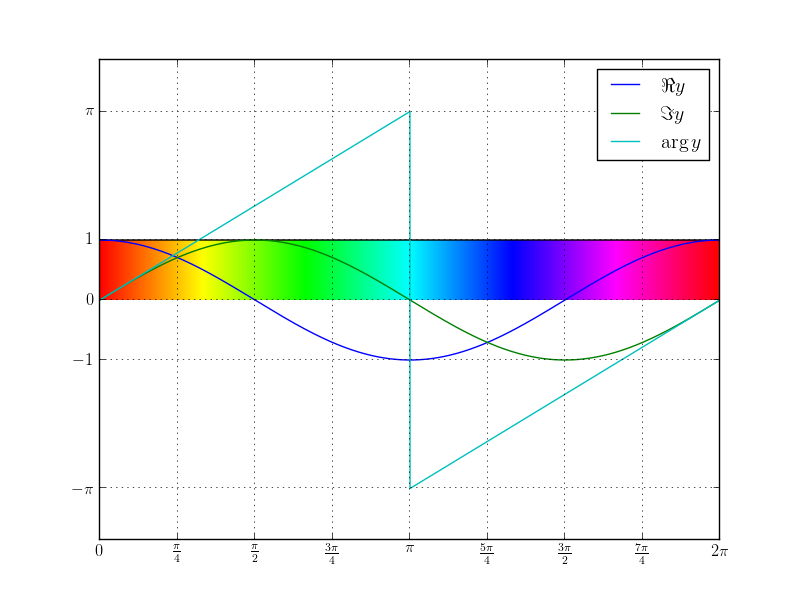
\includegraphics[width=\linewidth]{./fig/color_legend.png}
  \caption{This plot shows a complex-valued function $f:\mathbb{R}\rightarrow\mathbb{C}$
           in colour-coded fashion as well as the real and imaginary parts and the phase.}
  \label{fig:color_legend}
\end{figure}


\begin{figure}
  \centering
  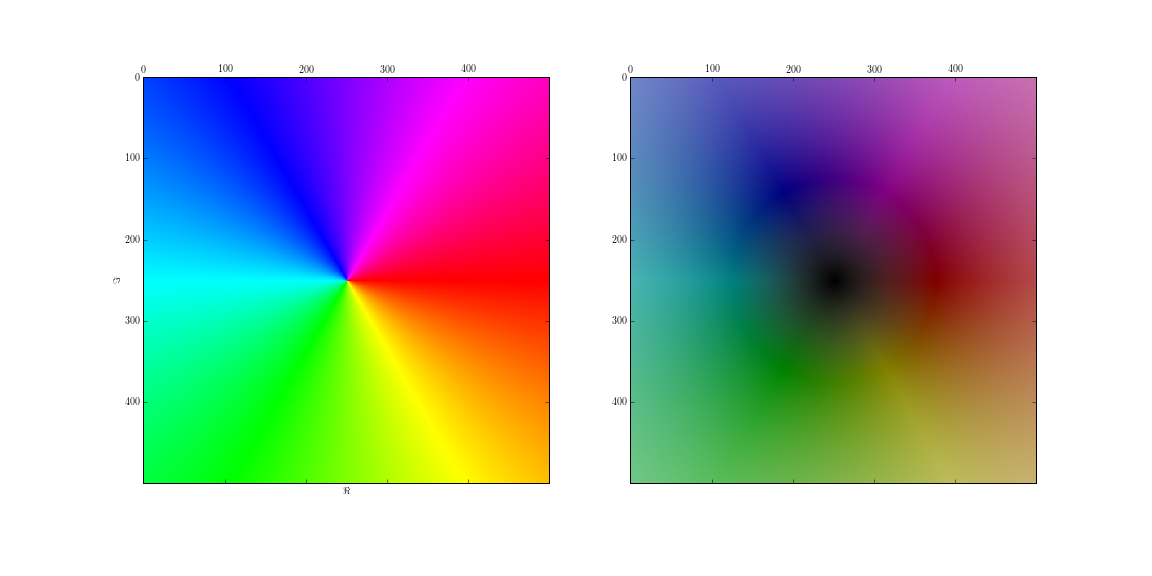
\includegraphics[width=\linewidth]{./fig/color_code.png}
  \caption{This plot shows the colour distribution for complex numbers $z$.}
  \label{fig:s}
\end{figure}

Sometimes one also darkens the colours depending on the magnitude of the
absolute value. For details about this see the given reference.
